\taskpic{ Положительно заряженная частица движется в однородных и
  взаимно перпендикулярных электрическом и магнитном полях. В
  некоторый момент времени её скорость равна $\vec{v}_0$ ($\vec{v}_0
  \perp \vec{E}$ и $\vec{v}_0 \perp \vec{B}$). Чему будет равна
  величина скорости частицы в те моменты времени, когда вектор её
  скорости будет составлять $180^{\circ}$ с вектором $\vec{v}_0$, при
  условии что $E = v_0 B$? Поле тяжести не учитывать.}
{
  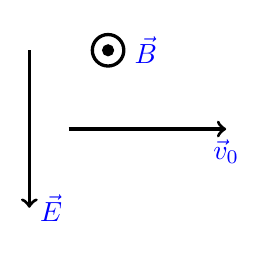
\begin{tikzpicture}
    \draw[very thick,->] (0,2) -- (0,0) node[right,blue] {$\vec{E}$};
    \draw[very thick,->] (0.5,1) -- (2.5,1) node[below,blue]
    {$\vec{v}_0$};
    \draw[very thick] (1,2) circle (0.2cm) node[right=0.2cm,blue] {$\vec{B}$};
    \draw[fill=black] (1,2) circle (0.07cm); 
  \end{tikzpicture}
}
% Квант, практикум абитуриента, 1999-3